\documentclass[11pt]{article}
\usepackage{deauthor,graphicx,times}
\usepackage[utf8]{inputenc}
\usepackage{algorithm}
\usepackage{algorithmic}
\usepackage[noend]{algpseudocode}

\graphicspath{{submissions/debaising_grid_search/figs/}}
\begin{document}
\title{Using Product Meta Information For Bias Removal In E-Commerce Grid Search}

\author{
  Apoorva Balyan\\
  \texttt{Walmart Global Tech India} \\
  \texttt{Apoorva.Balyan@walmart.com}
  \and
  Atul Singh\\
  \texttt{Walmart Global Tech India} \\
  \texttt{Atul.Singh@walmart.com}
  \and
  Praveen Reddy Suram\\
  \texttt{Walmart Global Tech India} \\
  \texttt{Praveen.Suram@walmart.com}
  \and
  Deepak Arora\\
  \texttt{Walmart Global Tech India} \\
  \texttt{Deepak.arora1@walmart.com}
  \and
  Varun Srivastava\\
  \texttt{Walmart Global Tech India} \\
  \texttt{varun.srivastava@walmart.com}
}
\maketitle
\begin{abstract}
In e-commerce, product search plays a crucial role in helping customers discover and purchase products. Most IR algorithms focus on creating a relationship between product and customer intent. These techniques stand on two pillars of information primarily- first, what information the seller provides about a product i.e description, title, taxonomy etc, and second, the implicit feedback data that is collected from the search logs which comprises of millions of user activity events. This data is inherently biased in nature as the user activity is not only dependent on the quality of query-item match but also on how probable the user is to observe that item in the first place. In the IR theory and past research efforts, discounting based on position in evaluation methods have been introduced to address this bias. However, these bias reduction methods cannot be applied efficiently to e-commerce cases because of the difference in the search results displayed to the user. The user behaviour in the list view search differs from that in the grid view search and is composed of three major factors- (1) middle bias (2) slower decay (3) row skipping.
There have been efforts to model the user attention probability in a grid-based search. However, these efforts have not been considered item meta-information hence, we propose a method to incorporate the item attributes in the user attention estimation model. The idea is to add a non-positional aspect in the propensity model of the user behaviour patterns. This is based on a simple argument that the user attention is not only dependent on the row and column of the item(aka position) but also on the features of product tile. These features can be shipping promise, price, reviews, ratings etc. Some of these feature tags have been designed to attract the attention of customers. Through various experiments on Walmart search logs data, We show that the proposed framework outperforms the debias baseline algorithms. The results reflect better on how different taxonomies, product categories can impact the user behaviour in grid-based product search.  
\end{abstract}
\section{Introduction}
There is an inherent difference between traditional search engines and e-commerce or product search engines. In traditional search engines like Google, the search results are displayed in a list view  whereas in the e-commerce search engines like www.walmart.com, the results are displayed in a grid view. The difference in the display of search results can impact the customer's attention and behaviour. Researchers in a previous study \cite{10.1145/3308558.3313514} were able to show that in the Image Search Engine Result Pages(SERPs), the user's attention can be defined by three factors: (1) User's attention within a row is more in the middle, so there is a bias towards the products in the middle (2) Users tend to skip rows while scrolling on a SERP (3) The decay of user attention is slower in a grid view compared to list view, where the decay happens drastically. This idea was further applied in the e-commerce search \cite{10.1145/3394486.3403336} and developed an inverse propensity bias model to correct the learning to rank algorithm. While position/presentation of the products on a SERP has been considered in the modelling of the bias, the impact of the product's meta-information on the user attention has still not been addressed. 

Intuitively, the SERPs of the e-commerce search engines are not only different in the presentation but also in the fact that e-commerce is a marketplace which has a direct monetary benefit for the sellers maintaining the product information on the page. Thus, the information present for each product tile such as 'Top Picks', 'Reviews' and 'Ratings' would have a very strong impact on the customers navigating this web space to get the best product suited for their requirements. Figure 1 and 2 shows the difference in results displayed in list vs grid view on walmart web and application.

\begin{figure}[t!]
\vspace{5mm}
\hspace{-3cm}
   \centering
   
\includegraphics[bb= 0 0 105 225, valign=t]{submissions/debaising_grid_search/figs/walmart_app_px.jpg}
   \caption{List view on Walmart App}
   \centering
   
\includegraphics[bb= 0 0 300 188, valign=t]{submissions/debaising_grid_search/figs/walmart_web_px.png}
   \caption{Grid view on Walmart web}
%   \Description{}
\end{figure}

The impact of these qualitative product features on bias would be different for different categories of products. For example : On a category of Milk with clear intent, the new customer might not be exploring so much on the view presented whilst on a category of clothing, the user's attention would be influenced by these product tile tags as discussed above. Hence, we extend the framework to model the product meta-information like Ratings, Reviews, Shipping Promise in the propensity model. 
Incorporating these features into the model will show the impact on the features displayed on the product tile. To model these features, we use a scoring algorithm to assign a score to each product and this score in modelled with the propensity scoring model. Our aim is to learn a ranker and evaluate the impact of the model using an evaluation metric. We also look at the different product taxonomies like Entertainment, Fashion etc because the customer's intent is different in each product taxonomy. 
\newline
We organize the rest of the paper in the following way: Section 2 contains related work on grid based e-commerce search, Section 3 contains our proposed framework with details on how the item feature scores are calculated and how the propensity score for modelling is derived, Section 4 mentions the experimental settings, evaluation metric and the results, along with the dataset description, and Section 5 presents the conclusion and the future work. Each section is further divided into subsections.

\section{RELATED WORK}
We will start with a brief introduction of the background and knowledge on the prior research work for analyzing the differences in the user behavior patterns in the list view vs the grid view search, and how this behaviour pattern is used in the propensity score modelling with a brief introduction to LambdaMART ranker.
\subsection{GRID SEARCH USER BEHAVIOUR PATTERNS}
Products in an e-commerce are placed in different view as compared to the majority of search engines that show the list view for the results. The different placement of products leads to a change in the interaction mechanisms of items. Previously, a number of studies have been done on the user behaviour on image or grid search engines \cite{10.1145/3308558.3313514, 10.1145/3397271.3401146,10.1145/2072298.2072308}. All these studies focused on comparing the user interaction behaviour in grid search setting to list view display setting by using search logs and eye tracking methods. Important differences in user behaviour, user being more exploratory and more time spent by the user are some of the findings that were observed. We list the major findings in grid based search as follows:
\newline \textbf{(a) Middle Bias:} There exists a "middle position bias" in the user's examination behaviour. Customers allocate their attention more to the items placed in middle positions in a row. The probability of the user examining items placed on left and right corner in a grid search is less compared to the items in the center. In \cite{10.1145/3308558.3313514}, the researchers consider the dwell time as the factor which is defined as the examination duration of an image and they confirm the middle bias phenomenon. Also, the user behaviour at each position in a row follows normal distribution. Researchers have not used this phenomenon in Learning to rank models of e-commerce yet, and we do not consider it in this research because in the dataset that we use, the number of columns is less than 4 or 5, and our hypothesis is that there are other details in e-commerce search that draw the user attention. So, the middle bias phenomenon is not very effective here. 
\newline
\textbf{(b) Row Skipping:} The customers do not examine each and every product in a grid from top to bottom, they tend to skip some rows. Users ignore particular rows and directly jump to some distant rows. The probability of the users skipping the first row is very low as compared to the other rows. In \cite{10.1145/3394486.3403336}, row skipping bias in the user behavior was considered in getting an Unbiased Learning to rank model. The probability of the user skipping a particular row was considered as a bias factor when calculating the lambda gradient for a query. The observation was that the row skipping models performed better in taxonomies where user intent was very clear and users were looking for specific set of items. In such cases, users were probable to skip the rows.
\newline
\textbf{(c) Slower Decay:} In a list-view web SERP, the attention of the customer decays in monotonically decreasing fashion and is also dramatic but in grid-view, the decay is much slower. The user behavior in the grid search is more exploratory and there is more browsing as there are a lot of items displayed in a page and users don't have to go to next page to view the next set of items as in the list-view. This leads to the user spending more time in the grid search, concentrating on the items, and thus the decay is slow. In \cite{10.1145/3394486.3403336}, the slower decay user behaviour bias was considered in training unbiased learning to rank models.
\newline
These findings are incorporated and Normalized Discounted Cumulative Gain(NDCG) evaluation method is also changed based on grid view search user behaviour.    

\subsection{Click Models} 
A lot of prior work has been done on-click modelling in the web search by extracting useful information from search logs of any search engine, mainly the click data. Cascade click model is one of the widely adopted technique in list based search that takes multiple types of user feed backs into account and models the user behavior as a sequence of actions\cite{10.1145/3159652.3159732, 10.1145/1341531.1341545}. There are different types of biases in the click-models, mainly the position bias. Learning from biased data without taking them into consideration leads to a less effective ranking function. In another study, unbiased learning to rank model was introduced where position bias was considered. 
Inverse propensity weighting is a well known technique adopted to address any kind of bias and is used for unbiased learning \cite{10.1145/3159652.3159732}. Most of the work in this area assumes that the propensity scores are present in the logs and they study how to reduce the model variance while remaining unbiased. The unbiased learning-to-rank framework is different, because in that, the propensity is not explicitly logged and is buried in the user behavior data implicitly. Unbiased learning to rank does debiasing of the click data and uses it to train the ranker. Unbiased LambdaMART framework \cite{10.1145/3308558.3313447} was introduced for training an unbiased ranker by jointly estimating the biases at click positions and the biases at non-click positions.
\subsection{LambdaMART Ranker}

LambdaMART is a widely used Learning to rank algorithm to solve ranking problems in search engines. LambdaMART \cite{burges2010from, 10.1145/3077136.3080838, 10.1145/1273496.1273513} uses gradient boosting and the gradient function of the loss function is called lambda function. The minimization of the objective function is performed using the lambda function on the training dataset. In LambdaMART, the lambda gradient of any document is calculated as 
\begin{equation}
\lambda_{i} = \sum_{j:(d_i , d_j)}{}\lambda_{ij} - \sum_{j:(d_j , d_i)}\lambda_{ji}
\end{equation}
 $\lambda_{ij}$ is defined as following :
\[\lambda_{ij}=\frac{-2}{1+exp(2(f(x_i)-f(x_j)))}\big|\Delta_{ij}\big|\]

where $\lambda_{ij}$ is the lambda gradient defined on a pair of documents $d_i$ and $d_j$, $\sigma$ is a constant,f($x_i$) and f($x_j$) are the scores of the two documents given by LambdaMART, $\Delta_{ij}$ denotes the difference between NDCG scores if documents $d_i$ and $d_j$ are swapped in the ranking list.

\section{Item Propensity Scoring Model}
We will start with a brief introduction of the background and knowledge on propensity estimation and joint optimization within the learning to rank models. Then we provide description of the changes to the proposed propensity scoring model using item features.
\subsection{Estimating Propensity using Product Meta Information}  
We hypothesize that the user is not only influenced by the presentation of search query results but also with certain attributes or tags that have been designed to get customer's attention by sellers.
\newline We consider four such attributes about an item which can impact user attention:
\newline(1) \textbf{Two Day Shipping}: In the fast paced world that we are in currently, every user wants their favorite products to be delivered at the earliest. Users tend to compare delivery options with other online competitors and place their order accordingly. Thus, to get user attention on items that are eligible for super fast delivery, a message is shown on product tile that this item is eligible for delivery within 2 days.  Fig 3,4 shows a two day shipping tag for products in the result set.
\newline(2) \textbf{Ratings}:  Ratings are given by previous users to the products on any e-commerce platform to indicate how satisfied or dissatisfied previous customers were for that product. This attributes tells what their experience was like and how they rate that experience on a scale of 1 to 5. Fig 3,4 shows the rating tag for products in the result set. 
\newline(3) \textbf{Reviews}: Reviews is the number of reviews a product has received till date. Reviews is a factor in fetching the rating score for an item. Users are attentive towards number of reviews as well along with rating, as an item with a high rating and very low number of user reviews is highly biased. Products with significant number of reviews gains user trust for that products rating.
\newline(4) \textbf{Relative Price}: Price is an important information displayed to the user on the product tile. A set of expensive items for a query may not attract user attention and user may not look in details with much attention. This will counter the slower decay factor. With relative price score, we try to get the expensive and cheap products for a query that is displayed to user. This feature is the relative score among price of all products fetched in the recall set for a particular query. \newline
~\\Based on the above features, we estimate a score and experiment with it in the propensity model. In scoring method, We assign a binary value in the scoring functions for 2-day shipping, ratings and reviews. 

\begin{figure}[t!]
\vspace{-38mm}
   \centering
   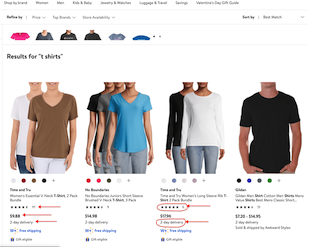
\includegraphics[bb = 0 0 240 185]{submissions/debaising_grid_search/figs/4-col-min.png}
   \caption{SERP with 4-column view with product meta information like Ratings, Reviews, Two day shipping}
   %\includegraphics[width=6cm, height=5cm]{figs/5-col-min.png}
\vspace{-13mm}
  \includegraphics[bb = 0 0 240 185]{submissions/debaising_grid_search/figs/5-col-min.png}
   \caption{SERP with 5-column view with product meta information like Ratings, Reviews, Two day shipping}
  % \Description{}
\end{figure}
According to the formulation: 
\begin{equation}
S(I) = \gamma\sum_{i=0}^3 K_i 
\end{equation}
where $K_i \epsilon [-1,1]$ represents binary vote of the item property. 
\newline How to assign the vote for score estimation of an item? To assign a vote for scoring, we look at the quantiles for item features in the data. The threshold for assigning a positive vote or a negative vote is decided using quantile values and then the final score is estimated by the summation of all the votes. The scoring algorithm is mentioned in Algorithm 1.
\newline For example: 
\newline If ratings $>$= 75th quantile-value, we assign a +1 score to the item or
If ratings $<$= 25th quantile-value, we assign a -1 score to the item etc. 
In this similar fashion, we compute a score for each item based on these features. 

\begin{algorithm}[H]
\caption{Score estimation using product meta information}
\begin{algorithmic}[1]
 \STATE Initialize $score_i$ as $0$
 \IF{$twoDayShipping_i>0.0$}
  \STATE $score_i \gets score_i + 1$
 \ENDIF
 \IF{$rating_i>=75thQuantileValue$}
  \STATE $score_i \gets score_i + 1$
 \ENDIF
 \IF{$rating_i<=25thQuantileValue$}
  \STATE $score_i \gets score_i - 1$
 \ENDIF
 \IF{$reviews_i>=75thQuantileValue$}
  \STATE $score_i \gets score_i + 1$
 \ENDIF
 \IF{$reviews_i<=25thQuantileValue$}
  \STATE $score_i \gets score_i - 1$
 \ENDIF
 \STATE $\Return \; score_i$
\end{algorithmic}
\end{algorithm}


\subsection{Changing the Slower Decay Model}			 
As mentioned before, in a SERP with a grid view the user attention decreases more slowly when compared to the results in a list view. According to the earlier work \cite{10.1145/3394486.3403336}, the probability of examination of an item at position, i is estimated as:
\begin{equation}
P(o^i = 1) = \prod_{j=0}^{i-1} min( \beta^{row(j)} * \alpha ), 1.0)
\end{equation}
where row(i) is the row-number for the item at position i, $\alpha$ is likeness of customer browsing the next item, $\beta$ models the customer's patience in grid view.
As we can see, the probability does not account for item meta-information shown on the item tile in SERP. If an user finds any item attractive in SERP, the user tends to spend more time on it and the probability of examination is more. There are multiple details shown on search page that may attract user attention viz. image quality or attractiveness, user ratings of that particular item, number of reviews on it, special offer tag, price of the product or the delivery date of the product. These factors will also contribute to the probability of user examining any particular product in Grid based SERP. Considering this, the decay factor will change accordingly. Based on this hypothesis, we model the estimated score above into the probability of examination at position, i as: 
\begin{equation}
P(o^i = 1) = \prod_{j=0}^{i-1} min( \beta^{row(j) +S(I)} * \alpha ), 1.0)
\end{equation}
\newline
We train a ranker f based on loss function L with the propensity score of slower decay model computed using $\alpha$, $\beta$ and $\gamma$ hyper parameters. We use LambdaMART with the ranker, gradient boosting trees as explained before. Following on the same lines, we calculate the lambda gradients by applying inverse propensity scoring. Hence, the lambda gradient for $k^{th}$ product can be re-written as:
\begin{equation}
\frac{\delta L}{\delta x_k} = \lambda_k = \sum_q\Bigg(\sum_{y_q^{i}=k\cap(i,j)\epsilon I_q} \frac{\lambda_{ij}}{P(o^i)} - \sum_{y_q^{i}=k\cap(j,i)\epsilon I_q} \frac{\lambda_{ij}}{P(o^j)}\Bigg)
\end{equation}
\newline
where i, j are the positions on the SERP, $x_q$ is the feature vector for query-product pair, $y_q^{i}$ means that the $k^{th}$ product is at position, i
and $\lambda_{ij}$ is defined as following :
\[\lambda_{ij}=\frac{-2}{1+exp(2(f(x_q^i)-f(x_q^j)))}\big|\Delta_{ij}\big|\]

$\Delta_{ij}$ is the value difference in the NDCG evaluation metric if i and j are to be swapped.
\newline
\newline
\textbf{Relative Price Feature : }
Price is another information displayed on the product tile in an E-commerce search. Most of the users have a budget in mind when they visit to shop any product. If ,for a particular query, most of the items in search results are expensive compared to the range user is looking for, the user may not spend much time on that query viewing the results thus the decay will be comparatively faster. Among the set of items displayed, if there is a relatively cheaper product that also has other attractive tile meta-information, the probability of examining it will be higher. 
As a part of this work, we consider relative price feature separately to observe the impact of the price on the user behaviour and to check if there is any price bias . Relative price calculation is done as follows: 
\begin{equation}
relp(i) = 1.0 - k * abs(func( log(x/mean\_price)))
\end{equation}

where relp(i) is the relative price score for an item i and x is the price of that particular item , k is a constant and mean\_price is the mean of prices of all items in the recall set of the query, abs is the absolute function to get the absolute value, func can be any activation function\cite{act} like tanh or sigmoid . For example , tanh is defined as 
\[tanh(x) = \frac{2}{1 + e^{-2x}} -1 \]
Sigmoid is defined as
\[sig(x) = \frac{1}{1 + e^{-x}} \]

Thus, in our dataset, we have the relative price score for all query-item pairs. Based on this, we redefine the probability of examination at position i in a GRID based SERP as 
\begin{equation}
P(o^i = 1) = \prod_{j=0}^{i-1} min( \beta^{row(j) +S(I) + \eta * relp(i)} * \alpha ), 1.0)
\end{equation}
\newline
where $\eta$ is the hyper-parameter introduced to tune the relative price feature in the slower decay model. 

For training slower decay model including price feature, we calculate the lambda gradient in the gradient function of LambdaMART as above in (7). 

\section{Experiments}

In this section, we conduct a series of experiments to compare our proposed method with the baseline methods for the removal of bias in grid-based e-commerce search. First, we explain our experimental settings, the datasets that we used, how we prepared them, and the metrics we used to evaluate the models. We then report the results obtained in our unbiased learning to rank setting.  

\subsection{Datasets}  
In this subsection, we provide a brief overview of the search log datasets that we used for our experiments. We used the data from the search logs of e-commerce website at Walmart, an American multinational retail corporation with a significant online presence. In particular, we use the data from three product taxonomies viz. Fashion, Entertainment (ENT), and Every Day Living (EDL), and by considering them for capturing and understanding the user behaviour and we eventually obtain four datasets, one for each category. Our datasets included queries, items, positions, and item features. The item features include raw features like item title match, item popularity, partial match score, along with engagement features like click rates, ‘add to cart’ rates, order rates and attribute features like the number of reviews, ratings, the relative price of the products among the recall set, and shipping promise.  

\subsection{Experimental Settings}
In this subsection, we describe the experimental setup. The most common way to evaluate the learning to rank model is by its performance on a holdout set that has unseen data. We perform experiments on each product taxonomy, as mentioned in the subsection above. In our datasets, we perform a random split into a training set (80\%), validation set (10\%), and test set (10\%). We carry out a fast grid search to obtain the best hyper-parameter values for the models. To keep the probability value in a reasonable range, we search alpha in \{0.8, 0.85 , 0.9 , 0.95\}, beta in \{1.05 , 1.1 , 1.15. 1.2\}, and gamma in \{0.001 , 0.003 , 0.005 , 0.007 , 0.01 , 0.03 , 0.05 , 0.07 , 0.1\}. For the LAMBDAMART ranker, we search for the learning rate in \{0.01 , 0.05 , 0.1\}, the maximum depth in \{3 , 5, 7\}, and the minimum data in leaf in \{20 , 30 , 40 , 50 , 60\}. We also tune for boosting fraction and feature fraction values in the range {0.7, 0.8, 0.9, 1.0} and {0.8, 0.9, 1.0} respectively. The other parameters are the default settings of Unbiased LambdaMART, while we keep the settings consistent for all the baseline and feature models. We consider the slower decay model[25] as the baseline method. Here, we optimize for the position 10 and consider the metric on the validation set to get the optimal parameter values. 

\subsection{Evaluation Metrics}
\begin{table}[b]
\centering
\begin{tabular}{|l|l|l|l|l|}
\hline
Taxonomy & $\alpha$ & $\beta$ & $\gamma$ \\
\hline
Fashion & 0.8 & 1.05 & 0.01 \\ 
\hline
EDL & 0.95 & 1.15 & 0.001 \\ 
\hline
ENT & 0.9 & 1.15 & 0.03\\ 
\hline
\end{tabular}
\caption{Tuned hyperparameters for item propensity scoring model for different taxonomies}
\end{table}

Here, we explain the evaluation metric considered for the experiment. We consider the traditional evaluation method of Information Retrieval Systems, Normalized Discounted Cumulative Gain (NDCG) as the evaluation metric \cite{10.1145/582415.582418, ndcg1, ndcg2}. Experiments are performed in offline settings and we obtain the NDCG metric at different positions to compare the proposed framework with the baseline method.
\begin{equation}
N D C G_k = \frac{D C G_k}{I D C G_k} 
\end{equation}

where 
\[I D C G_k = \sum_{i=1}^{|REL|} \frac{2^{rel_i} - 1}{\log_{2} (i+1)}\]


Here, IDCG@K  is the normalizer and $|REL|$ is the list of documents ordered by engagement in the set up to position k. To explain the slower decay of user attention we consider K = 1, 3, 5, 10 for the NDCGs.  

On the held-out dataset of Walmart Search logs, we calculate the prediction scores of our models. Using the prediction labels, we apply this evaluation method to get the metrics at different positions across different categories. 
\begin{table*}[t]
\begin{tabular}{|l|l|l|l|l|l|}
% \begin{table}[t]
% \centering
% \begin{tabular*}{\textwidth}{|l|l|l|l|l|} 
\hline
Taxonomy & Framework & NDCG$@$1 & NDCG$@$3 & NDCG$@$5 & NDCG$@$10 \\
\hline
Fashion (w/o price) & \begin{tabular}[c]{@{}l@{}}Benchmark Slower Decay\\Proposed framework\end{tabular} &
\begin{tabular}[c]{@{}l@{}}0.408\\\textbf{0.419}\end{tabular} & \begin{tabular}[c]{@{}l@{}}0.486\\\textbf{0.492}\end{tabular} & \begin{tabular}[c]{@{}l@{}}0.535\\\textbf{0.539}\end{tabular} & \begin{tabular}[c]{@{}l@{}}0.584\\\textbf{0.590}\end{tabular} \\ 
\hline
Fashion (with price) & \begin{tabular}[c]{@{}l@{}}Benchmark Slower Decay\\Proposed framework(with price)\end{tabular} &
\begin{tabular}[c]{@{}l@{}}0.408\\\textbf{0.420}\end{tabular} & \begin{tabular}[c]{@{}l@{}}0.486\\\textbf{0.494}\end{tabular} & \begin{tabular}[c]{@{}l@{}}0.534\\\textbf{0.540}\end{tabular} & \begin{tabular}[c]{@{}l@{}}0.583\\\textbf{0.590}\end{tabular}\\
\hline
Every Day Living & \begin{tabular}[c]{@{}l@{}}Benchmark Slower Decay\\Proposed framework\end{tabular} &
\begin{tabular}[c]{@{}l@{}}0.553\\0.553\end{tabular} & \begin{tabular}[c]{@{}l@{}}0.627\\\textbf{0.628}\end{tabular} & \begin{tabular}[c]{@{}l@{}}0.669\\0.669\end{tabular} & \begin{tabular}[c]{@{}l@{}}0.711\\0.711\end{tabular} \\ 
\hline
Entertainment & \begin{tabular}[c]{@{}l@{}}Benchmark Slower Decay\\Proposed framework\end{tabular} &
\begin{tabular}[c]{@{}l@{}}0.503\\0.503\end{tabular} & \begin{tabular}[c]{@{}l@{}}0.580\\\textbf{0.581}\end{tabular} & \begin{tabular}[c]{@{}l@{}}0.624\\0.624\end{tabular} & \begin{tabular}[c]{@{}l@{}}0.669\\\textbf{0.670}\end{tabular} \\ 
\hline
% \end{tabular*}
% \end{table}
\end{tabular}
\caption{Experimental Results on different taxonomies using held-out dataset.}
\end{table*}
\subsection{Experimental Results}

In this section, we provide an overview of the experimental results that we obtain. We share insights on: (1) how e-commerce search results get better with the proposed framework, and (2)how the user behaviour varies across the product taxonomies. We mention the results in Table 2 and summarize our observations as follows: 

\begin{itemize}
    \item Our proposed method for slower decay using product tile information outperforms the baseline method in Fashion vertical by significant margin. This clearly shows the effectiveness of our proposed framework and assumption that user attention decay is slower when user is attracted by any of the item features. 
    \item Performance of our proposed framework in Fashion affirms our initial assumption that users are more inclined on item tile information when shopping for clothing accessories and decay is much slower in such a case as user looks for detailed information. 
    \item The proposed framework of using item attributes in slower decay probability computation shows improvement in Entertainment and Every Day living category too compared to the baseline method of slower decay. Performance improvement is not much compared to Fashion, and this may be because the users have a specific intent when they shop in such categories. 
    \item Adding relative price feature in slower decay probability computation for fashion gave slight improvement over the proposed framework model without price feature.  This suggests that price is not a major factor in the users' attempt to click on that product and view the details. 
\end{itemize}
We train separate models for different taxonomies to show that the user behaviour patterns differ across categories and the users react differently to the product tile features. 
\newline
\newline
\textbf{Hyper Parameter Values:} 
Here, we report the values that we obtain for the hyper parameters ( $\alpha$ , $\beta$ , $\gamma$ ) and that achieve the optimal performance for the proposed framework.  For the Fashion category, the proposed slower decay model with $\alpha$ = 0.8, $\beta$ = 1.05 and $\gamma$ = 0.01 outperforms the others. Similarly, for the Every Day Living category, the proposed slower decay model with $\alpha$ = 0.95, $\beta$ = 1.15 and $\gamma$ = 0.001 works best. $\alpha$ = 0.9, $\beta$ = 1.15 and $\gamma$ = 0.03 are the optimal hyper-parameter values for the Entertainment category with the proposed slower decay framework. 
We experimented on Fashion with the price feature and $\alpha$ = 0.95 , $\beta$ = 1.15 , $\gamma$ = 0.05 , $\eta$ = 0.01 are the optimal hyper-parameter values for our dataset. 
\section{Conclusion and Future work}
In this paper, we tried to understand the impact of meta-information on the products displayed on the SERPs for user attention. We extended the solution of debiasing the grid product search by modelling the meta-information of the products, like rating, reviews, shipping promise, price in the propensity model. We showed through extensive experimentation how the different product taxonomies have different user behaviour.

As part of future work, we plan to extend this work to incorporate more product tile features and also use the image quality feature to model the user attention in Grid-based E-commerce search engines. We plan to try out different scoring methods as well for tile features score calculation and model middle bias , row skipping behaviour based on product tile features.

\begin{thebibliography}{10}
\itemsep=1pt
\begin{small}

\bibitem{10.1145/582415.582418} K.~J\"{a}rvelin and J.~Kek\"{a}l\"{a}inen. \newblock Cumulated Gain-Based Evaluation of IR Techniques. \newblock {\em ACM Trans. Inf. Syst}, 10.1145/582415.582418, 2002.

\bibitem{burges2010from} C.~JC Burges. \newblock From RankNet to LambdaRank to LambdaMART: An Overview. \newblock {\em https://www.microsoft.com/en-us/research/publication/from-ranknet-to-lambdarank-to-lambdamart-an-overview/}, MSR-TR-2010-82, 2010.

\bibitem{10.1145/1273496.1273513} Z.~Cao, T.~Qin, T.Y.~Liu, M.F.~Tsai and H.~Li. \newblock Learning to Rank: From Pairwise Approach to Listwise Approach. \newblock {\em Proceedings of the 24th International Conference on Machine Learning}, 10.1145/1273496.1273513, 2007.

 \bibitem{10.1145/3308558.3313447} Z.~Hu, Y.~Wang, Q.~Peng and H.~Li. \newblock Unbiased LambdaMART: An Unbiased Pairwise Learning-to-Rank Algorithm. \newblock {\em The World Wide Web Conference}, 10.1145/3308558.3313447, 2019.

\bibitem{10.1145/3308558.3313514} X.~Xie, J.~Mao, Y.~Liu, M.~de Rijke, Y.~Shao, Z.-Ye, M.~Zhang, S.~Ma. \newblock Grid-Based Evaluation Metrics for Web Image Search. \newblock {\em The World Wide Web Conference}, 10.1145/3308558.3313514, 2019.

\bibitem{10.1145/3394486.3403336} R.~Guo, X.~Zhao, A.~Henderson, L.~Hong and H.~Liu. \newblock Debiasing Grid-Based Product Search in E-Commerce. \newblock {\em AProceedings of the 26th ACM SIGKDD International Conference on Knowledge Discovery and Data Mining},1 0.1145/3394486.3403336, 2020.

\bibitem{10.1145/3159652.3159732} X.~Wang, N.~Golbandi, M.~Bendersky, D.~Metzler and M.-Najork. \newblock Position Bias Estimation for Unbiased Learning to Rank in Personal Search. \newblock {\em Association for Computing Machinery}, 10.1145/3159652.3159732, 2018.

\bibitem{10.1145/2072298.2072308} B.~Geng, L.~Yang, C.~Xu, X.S.~Hua and S.-Li. \newblock CThe Role of Attractiveness in Web Image Search. \newblock {\em AProceedings of the 19th ACM International Conference on Multimedia}, 10.1145/2072298.2072308, 2011.

\bibitem{10.1145/3397271.3401146} X.~Xie, J.~Mao, Y.~Liu, M.~de Rijke, H.~Chen, M.~Zhang, S.~Ma. \newblock Preference-Based Evaluation Metrics for Web Image Search. \newblock {\em Proceedings of the 43rd International ACM SIGIR Conference on Research and Development in Information Retrieval}, 10.1145/3397271.3401146, 2020.

\bibitem{10.1145/1341531.1341545} N.~Craswell, O.~Zoeter, M.~Taylor and B.~Ramsey. \newblock CAn Experimental Comparison of Click Position-Bias Models. \newblock {\em Proceedings of the 2008 International Conference on Web Search and Data Mining}, 10.1145/1341531.1341545, 2008.

\bibitem{10.1145/3077136.3080838} S K.~K.Santu, P.~Sondhi and C.~Zhai. \newblock On Application of Learning to Rank for E-Commerce Search. \newblock {\em Proceedings of the 40th International ACM SIGIR Conference on Research and Development in Information Retrieval}, 10.1145/3077136.3080838, 2017.

\bibitem{ndcg1} Sham.~S. \newblock Discounted Cumulative Gain. \newblock {\em https://machinelearningmedium.com/2017/07/24/discounted-cumulative-gain/}, 2017.

\bibitem{ndcg2} Chandekar.~Pranay. \newblock Evaluate your Recommendation Engine using NDCG. \newblock {\em ttps://towardsdatascience.com/evaluate-your-recommendation-engine-using-ndcg-759a851452d1}, 2020.

\bibitem{act} A.~Sharma V. \newblock Understanding Activation Functions in Neural Networks. \newblock {\em https://medium.com/the-theory-of-everything/understanding-activation-functions-in-neural-networks-9491262884e0}, 2017.
\end{small}
\end{thebibliography}

\end{document}
